\section{Metodologias para a construção de ontologias}

\subsection{Método Cyc}

 \textit{CyC} é um projeto do \textit{Microelectronics and Technology Computer Corporation (MCC) em Austin, Texas},
 que fornece uma base para o raciocínio de senso comum através do desenvolvimento de ontologias para uma ampla 
 variedade de aplicações específicas de domínio. Todo o conhecimento em CyC é representado de forma declarativa na 
 forma de afirmações em uma variante da lógica de primeira ordem chamado CYCL. A própria base de conhecimento CYC 
 contém afirmações simples, motor de inferência pode ser usado para derivar novas afirmações que utilizam esta base
 de conhecimento.
 
As ontologias subjacentes CYC são organizados em conjuntos de módulos conhecidos como microteorias. Cada microteoria
captura o conhecimento e o raciocínio necessário para algumas de domínio particular, como espaço, tempo, causalidade,
ou agentes.

Podem existir múltiplos microteorias para um determinado domínio, refletindo as diferentes perspectivas e suposições
feitas para pessoas modelar esse domínio. Neste sentido, CYC não é uma ontologia integrado monolítica, ao contrário,
é uma rede de microteorias para um conjunto de domínios cuja união abrange os diferentes compromissos da ontologia que
podem ser feitas dentro desses domínios \cite{Andreia2010}.

A Figura \ref{fig:processos_cyc} ilustra os três processos que foram conduzidos no desenvolvimento da
base de conhecimento Cyc em 1990 por Douglas Lenat e Ramanathan Guha
(\textit{apud} \citeauthor{DanielaLucas2008}, \citeyear{DanielaLucas2008}).

\begin{figure}[h] 
\centering 
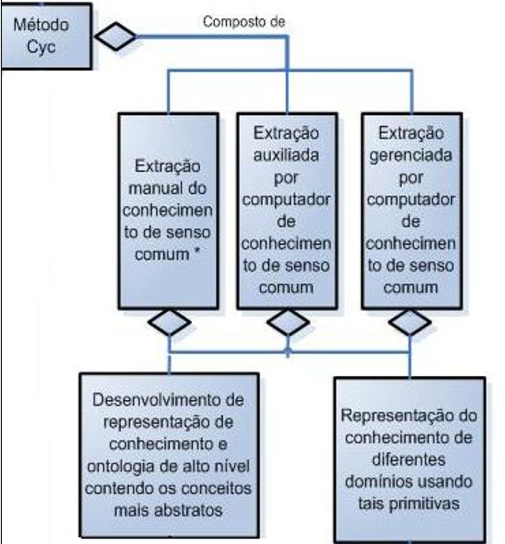
\includegraphics[scale=0.6]{Figuras/1.png} 
\caption[Processos e atividades propostas pelo método Cyc]
{Processos e atividades propostas pelo método Cyc. Fonte: \cite{DanielaLucas2008}}
\label{fig:processos_cyc}
\end{figure}

\begin{figure}[h] 
\centering 
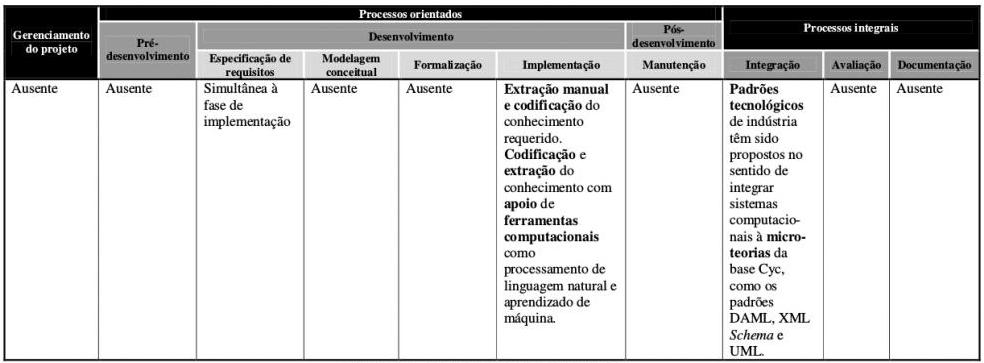
\includegraphics[scale=0.3]{Figuras/2.png}
\caption[Tabela abreviada do método Cyc]{Tabela abreviada do método Cyc. Fonte: \cite{DanielaLucas2008}}
\end{figure}

% \subsection{Metodologia de Gruninger e Fox}    
% 
%  Esta metodologia baseia-se na experiência em desenvolvimento de ontologia do projeto Tove dentro do domínio de processos e atividades de negócios de
% modelagem. Essencialmente, ele envolve a construção de um modelo lógico de o conhecimento que está a ser especificado por meio da ontologia. Este modelo não é construído diretamente. Primeiro, uma descrição informal é feita das especificações para
% serem atendidas pela ontologia e, em seguida, esta descrição é formalizada. As medidas propostas são as seguintes:
% 
% \begin{enumerate}
%  \item Captação de cenários motivadores;
%  \item Formulação de perguntas informais de competência;
%  \item Especificação da terminologia da ontologia dentro de uma linguagem formal:
%   \subitem Obtendo terminologia informal;
%   \subitem Especificação da terminologia formal;
%  \item Formulação de questões formais de competência usando a terminologia da ontologia.
%  \item Especificação de axiomas e definições para os termos na ontologia dentro da linguagem formal.
%  \item Estabelecer condições para a caracterização da integralidade da ontologia.
%   \subitem Ontologias desenvolvida utilizando esta metodologia.
%   \subitem Aplicações utilizando ontologias desenvolvida com esta metodologia.
%   \subitem Empresa Projeto Workbench.
%   \subitem Abastecimento Integrado Cadeia Project Management agentes.
%   \subitem Análise da metodologia.\cite{VariosAutores2009}
% \end{enumerate}
% 
% \pagebreak
% 
% A Figura \ref{fig:procedimentos_gruninger} ilustra tal metodologia:
% 
% \begin{figure}[h] 
% \centering
% 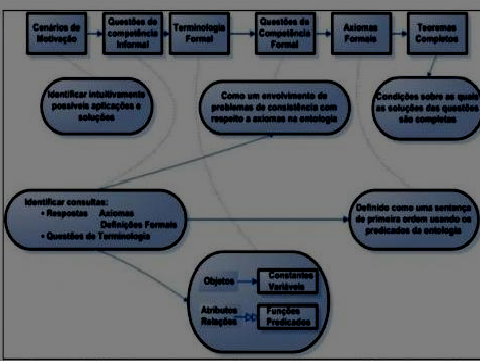
\includegraphics[scale=0.65]{Figuras/3.png}
% \caption[Procedimentos propostos na metodologia de Gruninger e Fox]
% {Procedimentos propostos na metodologia de Gruninger e Fox. Fonte: \cite{DanielaLucas2008}}
% \label{fig:procedimentos_gruninger}
% \end{figure}
% 
% \begin{figure}[h] 
% \centering
% 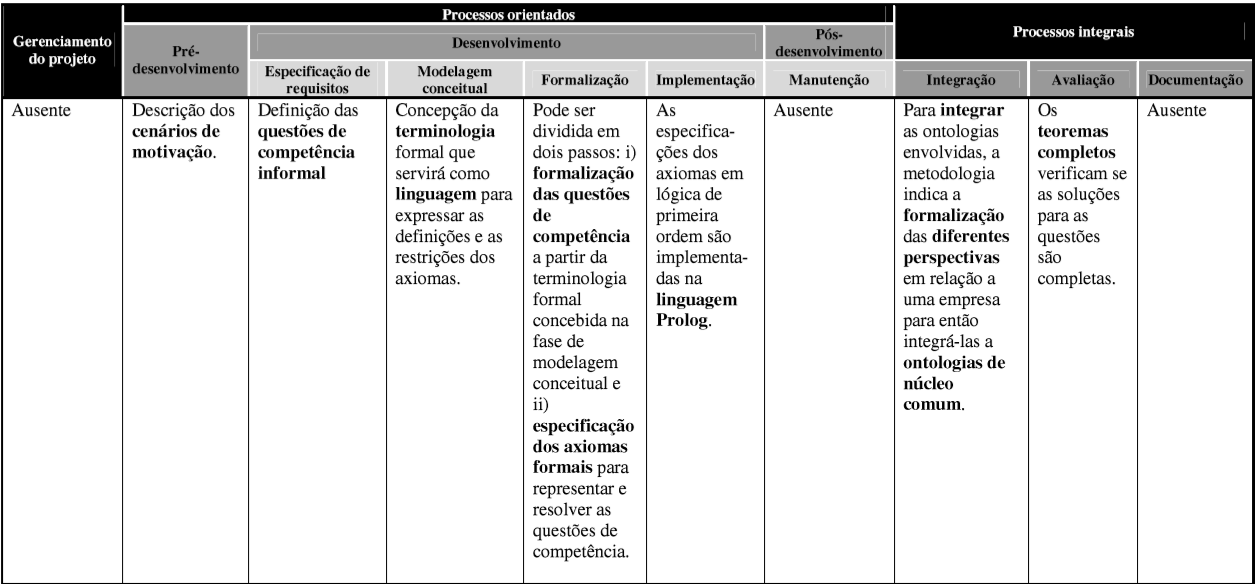
\includegraphics[scale=0.3]{Figuras/4.png}
% \caption[Tabela abreviada da metodologia de Gruninger e Fox]{Tabela abreviada da metodologia de Gruninger e Fox. Fonte: \cite{DanielaLucas2008}}
% \end{figure}
%  
% \subsection{Método de Uschold e King} 
%  Uschold apresenta uma metodologia unificada, combinando as "melhores" partes de OE e Tove em um unificado
%  método (apud Uschold, 1996). O primeiro passo é definir a finalidade da ontologia, ou seja, porque é a ontologia sendo
%  construída. Isto pode ser feito de várias maneiras, por exemplo para identificar os utilizadores destinados, ou como no
%  projeto com Tove, cenários de motivação e perguntas de competência, ou um documento de requisitos do usuário. Em seguida,
%  o desenvolvedor deve decidir o nível de formalidade que a ontologia tem que ter. Na próxima fase, o desenvolvedor precisa
%  encontrar os conceitos que deveriam estar na ontologia e as relações entre eles. Uschold prefere ir pelo means-out maneira
%  ao definir termos e relacionamentos. Quando se trata de construir a ontologia o autor descreve quatro diferentes abordagens.
%  O primeiro deles é pular as etapas anteriores e usar um editor de ontologias para definir
%  os termos e axiomas \cite{SeveralAuthorUFF2011}.
% 
% Em segundo lugar, fazer os passos anteriores e, em seguida, iniciar uma codificação formal. A terceira abordagem é produzir
% um documento intermediário que consiste em os termos e definições que apareceram na etapa anterior, este documento pode ser
% o resultado final, ou seja especificação do código formal ou documentação para ele ser. O quarto e aproximação final é
% identificar os termos formais a partir do conjunto de termos informais. A parte final presente no Uschold é o ciclo de
% avaliação ou a revisão, onde a ontologia desenvolvida é comparada com as questões da competência ou as necessidades
% dos utilizadores \cite{SeveralAuthor2011}.
% 
% A Figura \ref{fig:estagios_uschold_king} apresenta tais estágios envolvidos na construção de uma ontologia:
% 
% \begin{figure}[h] 
% \centering 
% 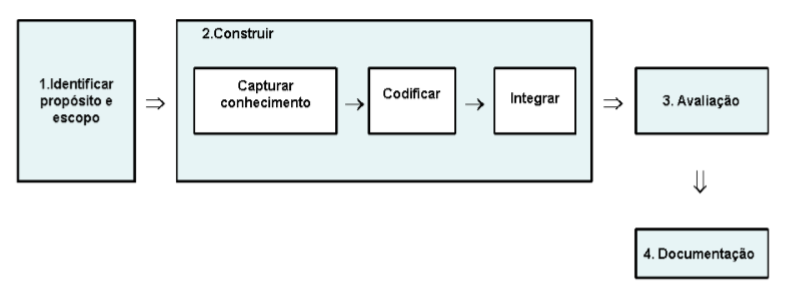
\includegraphics[scale=0.5]{Figuras/5.png}
% \caption[Estágios do método de Uschold e King]{Estágios do método de Uschold e King. Fonte: \cite{DanielaLucas2008}}
% \label{fig:estagios_uschold_king}
% \end{figure}
% 
% \pagebreak
% 
% \begin{figure}[h] 
% \centering 
% 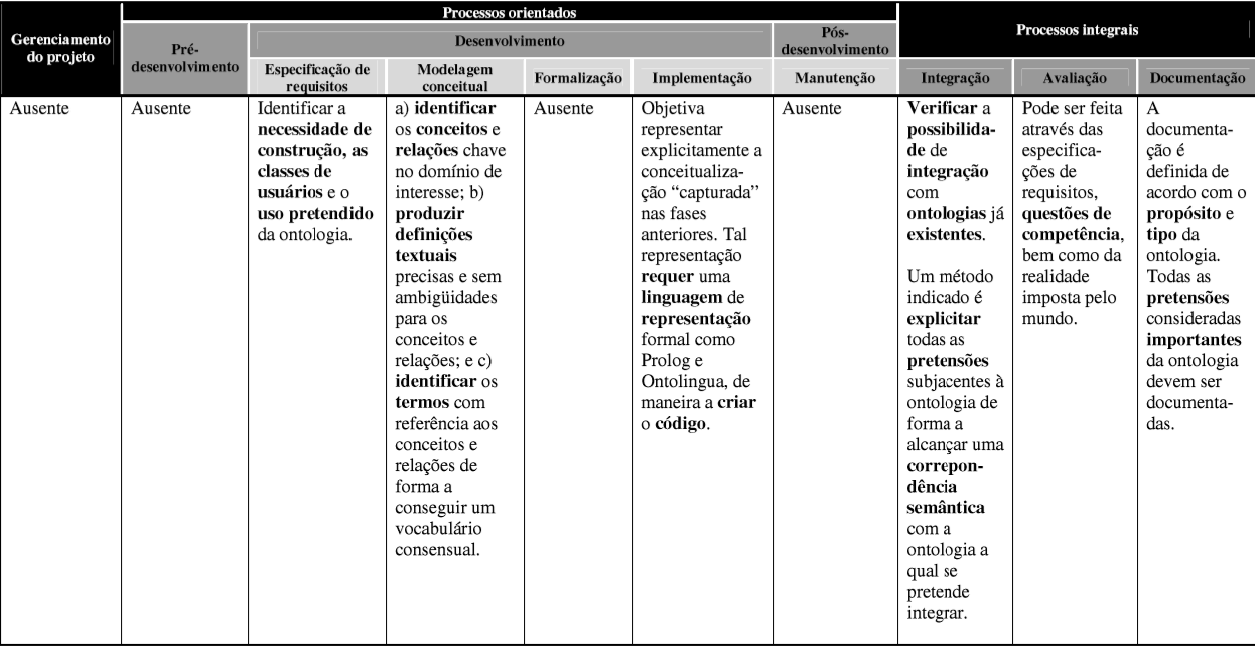
\includegraphics[scale=0.3]{Figuras/6.png} 
% \caption[Tabela abreviada do método de Uschold e King]{Tabela abreviada do método de Uschold e King. Fonte: \cite{DanielaLucas2008}}
% \end{figure}
% 
% \subsection{Método Kactus} 
%  Kactus é um método amplamente utilizado para o desenvolvimento de sistemas baseados em conhecimento, em que ontologias
%  desempenham um papel importante. O projeto Kactus foi um projecto de acompanhamento que centrou-se na questão do
%  desenvolvimento da ontologia. Uma abordagem de engenharia é adotada, salientando design modular, redesenhar e reutilizar.
%  Uma ontologia é construída a partir de uma biblioteca de ontologias de pequena escala, que requer mapeamento entre as várias
%  ontologias incluídas na desenvolvimento da nova ontologia. Dois tipos de funções de mapeamento são definidas entre o
%  vocabulários de ontologias:
%  
% (I) não há nenhuma mudança na semântica de expressões da ontologia mapeada.
% (II) uma alteração ocorre na semântica da ontologia mapeada como uma interpretação do que ocorre.
% 
% A seleção de ontologias relevantes a partir de uma biblioteca é suportado por um esquema de indexação para ontologias.
% Este caracteriza o contexto interpretação da utilização de uma ontologia segundo três dimensões: tipo de tarefa; método
% de resolução de problemas, e do tipo de domínio. O modular princípio de desenvolvimento é comum em engenharia ontológica
% e decorre do foco na reutilização. Embora o trabalho em funções de mapeamento está atualmente bastante limitado, a
% abordagem parece ter potencial em alfaiataria, ontologias para aplicação particular \cite{VariosAutores2009}. 
% 
% \pagebreak
% 
% \begin{figure}[h] 
% \centering 
% 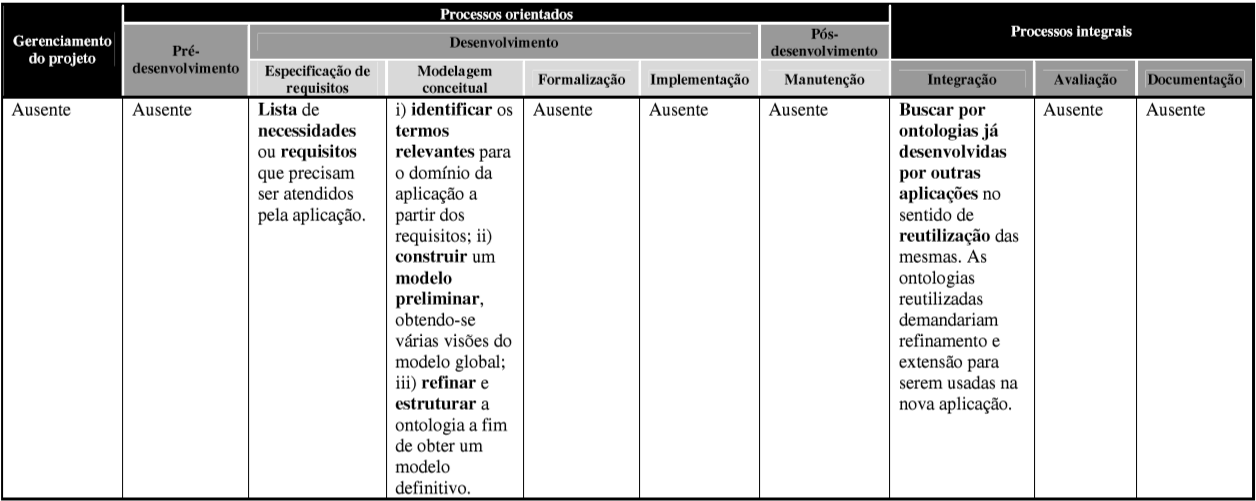
\includegraphics[scale=0.4]{Figuras/7.png} 
% \caption[Tabela abreviada do método Kactus]{Tabela abreviada do método Kactus. Fonte: \cite{DanielaLucas2008}}
% \end{figure}
%  
% \subsection{Metodologia Methontology} 
%  
%  A metodologia METHONTOLOGY é utilizada para construir ontologias a partir do zero 
%  (FERNANDÉZ et al., 1997 \textit{apud} \citeauthor{}, \citeyear{}).
%  O primeiro passo é especificar a finalidade da ontologia, o nível de formalidade e do escopo da ontologia.
%  Em seguida, todo o conhecimento precisa ser coletado. Existem várias maneiras de fazer isso: através de \textit{brainstorming},
%  entrevistas estruturadas e não estruturadas, análise formal e informal de textos e ferramentas de aquisição de conhecimento.
%  Na fase de conceituação Fernández  primeiro propos a construção de um glossário de termos de todo o conhecimento
%  possivelmente útil no domínio determinado. Em seguida, os termos são agrupados de acordo com conceitos e verbos,
%  e estes são reunidos para formar tabelas de fórmulas e regras. A próxima coisa a fazer é verificar se existem quaisquer
%  ontologias já existentes que podem e devem ser usados. O resultado da fase de implementação é a ontologia codificada em 
%  uma linguagem formal, que pode ser avaliada (verificados e validados) de acordo com algumas referências. A parte final
%  consiste na documentação \cite{VariosAutores2009}.
%  
% Cada fase resulta em um documento que descreve a ontologia desenvolvida até agora. Durante o ciclo de vida temos a
% atividade de suporte. E nela se engloba a aquisição do conhecimento, documentação e avaliação conforme pode ser visto
% na figura \ref{fig:estagios_methontology}:
% 
% \begin{figure}[h] 
% \centering
% 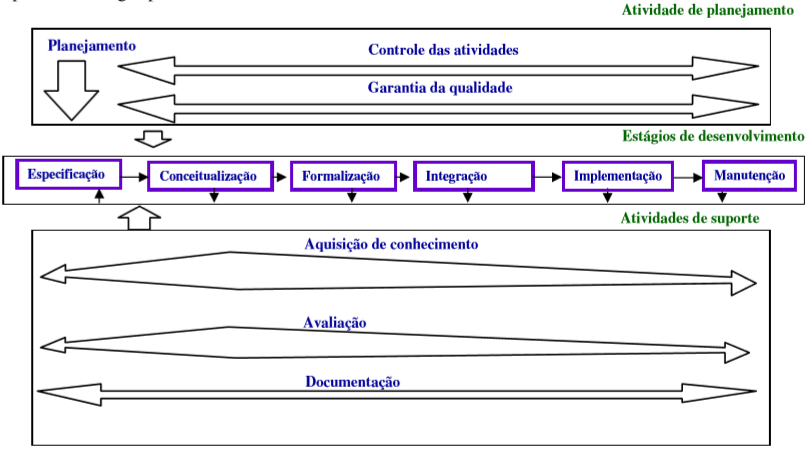
\includegraphics[scale=0.5]{Figuras/8.png} 
% \caption[Estágios e atividades do ciclo de vida da ontologia]
% {Estágios e atividades do ciclo de vida da ontologia. Fonte: \cite{DanielaLucas2008}}
% \label{fig:estagios_methontology}
% \end{figure}
% 
% \pagebreak
% 
% \begin{figure}[h] 
% \centering 
% 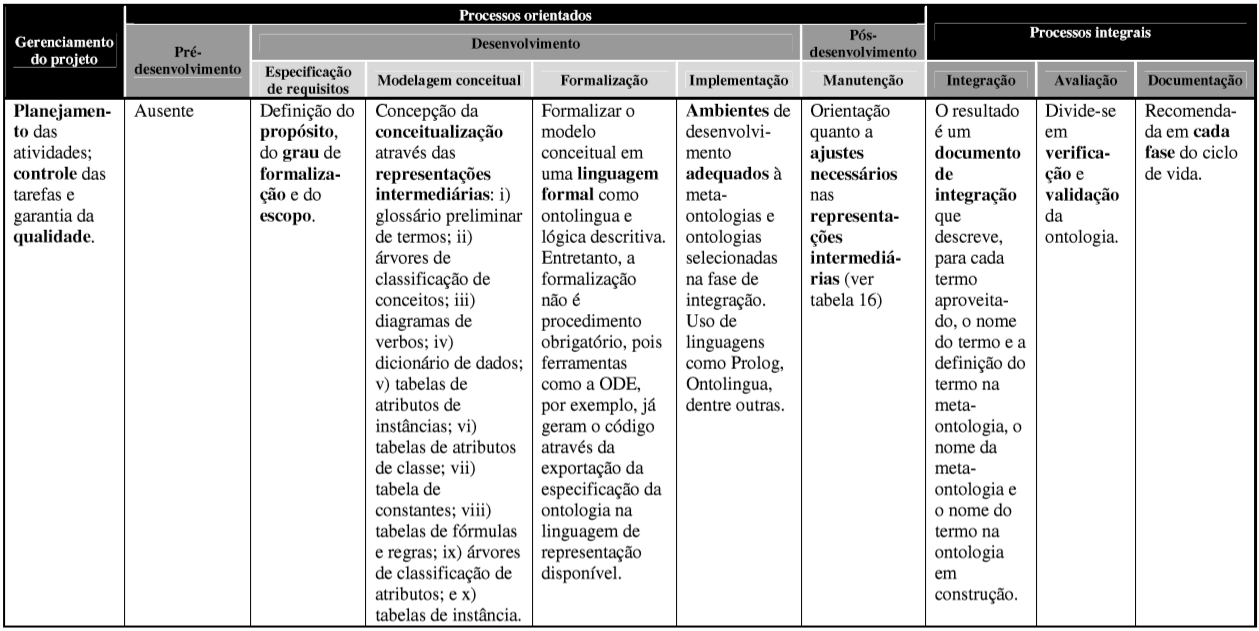
\includegraphics[scale=0.4]{Figuras/9.png} 
% \caption[Tabela abreviada da metodologia Methontology]
% {Tabela abreviada da metodologia Methontology. Fonte: \cite{DanielaLucas2008}}
% \end{figure}
%  
% \subsection{Método Sensus} 
%  O método baseado na Sensus é uma abordagem top-down para derivar ontologias específicas de domínio de grandes ontologias.
%  As etapas são as seguintes:
%  
%   1) Uma série de termos são tomados como semente;\newline
%   2) Esses termos de sementes estão ligados à mão para SENSUS;\newline
%   3) Todos os conceitos no caminho dos termos de sementes para a raiz SENSUS estão incluídos;\newline
%   4) Termos que poderiam ser relevantes no domínio e não têm ainda aparecido são adicionados;\newline 
%   5) Finalmente, para os nós que têm um grande número de caminhos através deles,
%   toda a subárvore sob o nó é adicionado às vezes, baseada na idéia de que, se muitos dos gânglios em uma sub-árvore,
%   foram encontrados para ser relevante, em seguida, os outros nós na sub-árvore é provável que sejam relevantes.
%   Esta metodologia utiliza a ontologia existente, onde a fusão será complexa devido a diferentes estruturas \cite{SeveralAuthorUFF2011}.
% 
% \begin{figure}[h] 
% \centering 
% 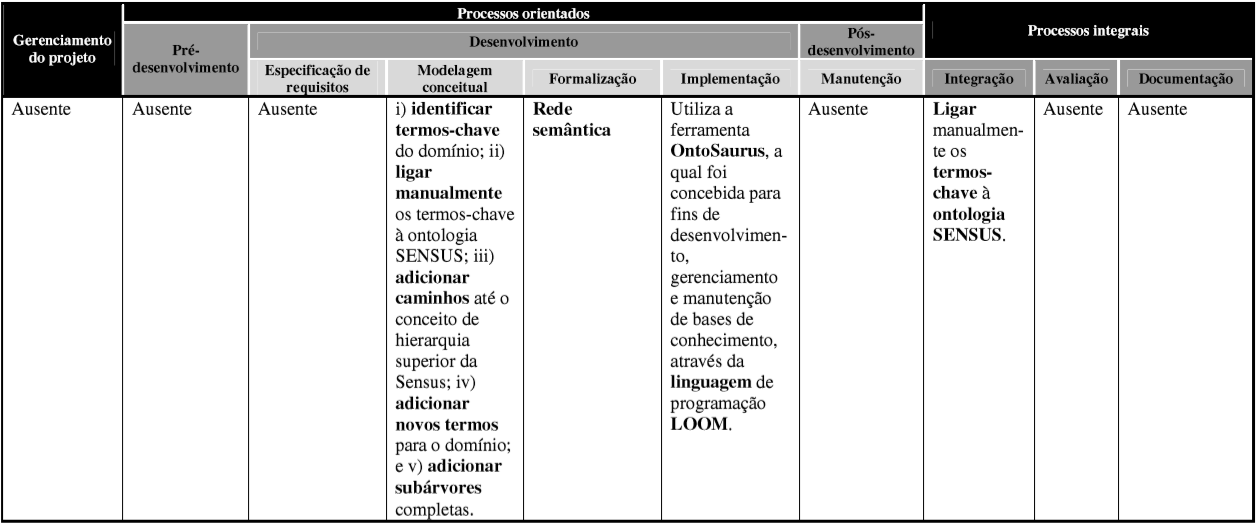
\includegraphics[scale=0.4]{Figuras/10.png} 
% \caption[Tabela abreviada do método Sensus]{Tabela abreviada do método Sensus. Fonte: \cite{DanielaLucas2008}}
% \end{figure}

\subsection{Método 101} 
 O método 101 foi criado por  Natalya F. Noy e Deborah L. McGuinness com base em experiências no desenvolvimento
 das ontologias de alimentos e vinhos, utilizando para isso o conceituadissimo software para a criação e edição de
 ontologias o Protégé-2000. Noy e McGuinness (2001, p.2) disseram em sua obra que não existe uma única maneira mais
 adequada para a construção de ontologias, e portanto não definiriam a melhor ontologia. A idéia desse método surgiu
 quando as autoras tiveram a idéia de compartilhar  as suas experiências para a construção de ontologias, de modo a
 ser útil em algum momento para outras pessoas, em outros projetos. A origem do método segundo as autoras foram baseadas
 na literatura do POO (paradigmas orientados a objetos), contudo para o desenvolvimento de ontologias cada um deles, é
 claro, tem as suas particularidades, diferindo em alguns aspectos. \cite{VariosAutores2009} Para a execução do método 101,
 sete passos são considerados fundamentais no processo de construção da ontologia, conforme mostrado na figura \ref{fig:processo_101}.

\begin{figure}[h] 
\centering 
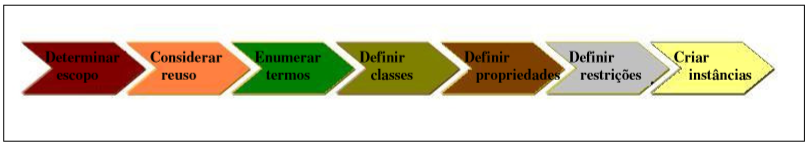
\includegraphics[scale=0.6]{Figuras/11.png} 
\caption[Processo de desenvolvimento de ontologias.]{Processo de desenvolvimento de ontologias. Fonte: \cite{DanielaLucas2008}}
\label{fig:processo_101}
\end{figure}

\begin{figure}[h] 
\centering 
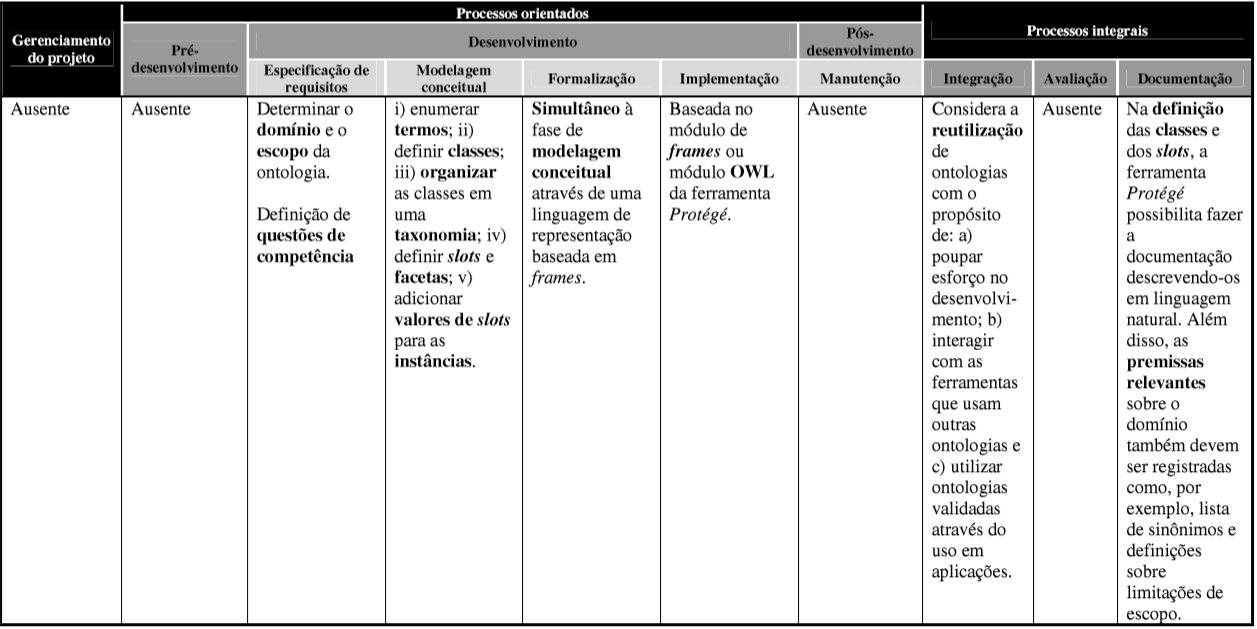
\includegraphics[scale=0.4]{Figuras/12.png} 
\caption[Tabela abreviada do método 101]{Tabela abreviada do método 101. Fonte: \cite{DanielaLucas2008}}
\end{figure}


  A partir da análise conceitual dos métodos e metodologias para construção de ontologias presentes na sessão anterior, 
  o método escolhido para a realização deste projeto, levando em conta as etapas/fases propostas por cada uma dessas 
  metodologias ou métodos no que tange ao processo de construção de ontologias, foi o método \textit{\textbf{Ontology 101}}.
  
  Os aspectos observados na escolha do método foram: \textbf{a)} suporte literário bem consolidado e disponível 
  (livros, artigos, guias e etc); \textbf{b)} o método é baseado na literatura do paradigma orientado a objetos;
  \textbf{c)} familiarização por parte dos integrantes do grupo com os conceitos e processos propostos pelo método.

\vspace{0.5cm}
  
{\raggedright
  \textit{\textbf{Ontology 101}}.
}
  
  De acordo com Breitman (\citeyear{breitman05}), o processo de construção de uma ontologia a partir do método 101,
  resumidamente, envolve as seguintes etapas:
  \begin{itemize}
   \item Definição das classes dessa ontologia;
   \item Disposição das classes em uma hierarquia taxonômica;
   \item Definição de propriedades e valores para os mesmos;
   \item Preenchimento dos valores das propriedades para cada instância.
  \end{itemize}
  
  \begin{figure}[!htb]
    \centering
    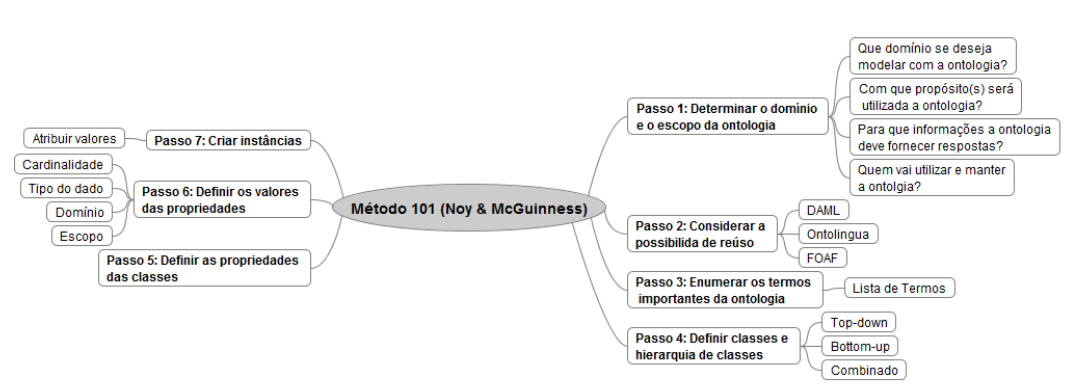
\includegraphics[scale = 0.4]{101-Web}
    \caption[Método 101 para construção de ontologia]{Método 101 para construção de ontologias. Fonte: \cite{bortolato14}}
    \label{fig:101-Web}
  \end{figure}
  
  A Figura \ref{fig:101-Web} ilustra um esquemático do método 101 no qual é detalhado cada um dos seus sete passos.
  
\vspace{0.5cm}  
  
{\raggedright  
  \textbf{1º Passo: Determinar o domínio e o escopo da ontologia}
}
  
  Para se determinar o domínio e o escopo da ontologia, Natalya F. Noy e Deborah McGuinness sugerem os seguintes questionamentos
  \cite{breitman05}:
  
  \begin{itemize}
   \item Que domínio se deseja cobrir com a ontologia?
   \item Com que protótipo(s) será utilizada a ontologia?
   \item Para que informações a ontologia deve fornecer respostas?
   \item Quem vai utilizar e manter a ontologia?
  \end{itemize}
  
  Segundo Breitman (\citeyear{breitman05}), estas perguntas servirão para avaliar a ontologia após sua conclusão.
  
\vspace{0.5cm}  
  
{\raggedright  
  \textbf{2º Passo: Considerar o reúso de outras ontologias}
}
  
  É importante considerar os termos que alguém já codificou em uma ontologia e se é possível refinar ou reutilizar
  modelos existentes para o domínio de nossa própria aplicação. Várias ontologias estão disponíveis eletronicamente,
  podendo ser facilmente importadas para editores e ambientes de desenvolvimento. \cite{breitman05}
  
  Atualmente existem várias bibliotecas de ontologias que disponibilizam modelos para reúso. As bibliotecas do projeto
  Ontolingua, DAML e KACTUS, por exemplo, disponibilizam um grande número de ontologias que podem ser reutilizadas, refinadas
  ou adaptadas. \cite{breitman05}
  
\vspace{0.5cm}  
  
{\raggedright  
  \textbf{3º Passo: Enumerar os termos importantes da ontologia}
}
  
  É útil fazer uma lista de todos os termos que deseja-se definir ou explicar aos usuários. Quais termos gostaríamos de abordar? 
  Quais propriedades terão esses termos? O que gostaríamos de dizer sobre esses termos? É importante obter uma lista compreensiva 
  de termos sem se preocupar com a redundância entre os conceitos que eles representam, relacionamentos entre termos ou qualquer 
  propriedade que eles venham a ter. \cite{noy15}
  
\vspace{0.5cm}  
  
{\raggedright  
  \textbf{4º Passo: Definir classes e a hierarquia de classes}
}
  
  Segundo Noy e McGuinness (\citeyear{noy15}), definir as classes e a hierarquia entre elas e definir  suas propriedades (5º Passo)
  são feitos de forma paralela,  pois seria difícil fazer um após o outro. O curso natural, na prática, é definir uma classe e 
  descrever suas propriedades logo após.
  
  Existem muitas abordagens possíveis para se fazer uma hierarquia de classes: \cite{breitman05}
  
  \begin{itemize}
   \item A abordagem \textbf{topo-para-baixo} (\textit{top-down}) inicia-se com a definição dos conceitos mais gerais do domínio (pai ou superclasse) 
   e, posteriormente, esses conceitos são especializados em conceitos mais específicos (filhos ou subclasses). Essa abordagem é 
   conhecida, também, como decomposição funcional. 
   \item A abordagem \textbf{baixo-para-cima} (\textit{bottom-up}), pelo contrário, inicia-se com a definição dos conceitos mais específicos 
   (filhos ou subclasses) com o subsequente agrupamento dessas classes em conceitos mais gerais (pai ou superclasse). Esses
   agrupamentos são organizados de acordo com uma estratégia de generalização. \cite{noy15}
   \item A \textbf{Combinação} (\textit{middle-out}) é a conjunção das abordagens descritas anteriormente. Primeiramente, são definidos
   os conceitos mais notórios e então esses são especializados e generalizados adequadamente. \cite{noy15}
  \end{itemize}
  
  De acordo com Noy e McGuinness (\citeyear{noy15}), nenhuma das três abordagens é a melhor a ser utilizada, isso vai depender da visão
  pessoal do modelador do domínio. Geralmente, a \textbf{combinação} tende a ser a mais utilizada pelos desenvolvedores de ontologia,
  uma vez que os conceitos mais centrais são mais descritivos no domínio da ontologia. \cite{noy15}
  
\vspace{0.5cm}  
  
{\raggedright  
  \textbf{5º Passo: Definir as propriedades das classes}
}
  
  Segundo Noy e McGuinness (\citeyear{noy15}), as classes sozinhas não proveem subsídios suficientes para responder as questões de competência
  do 1º Passo (Determinar o domínio e o escopo da ontologia). Para isso é necessário criar uma estrutura interna de seus conceitos.
  
  No passo anterior (Definir classes e a hierarquia das classes) já fora selecionadas as classes obtidas dos termos que foram listados
  no 3º Passo (Enumerar os termos importantes da ontologia).  Muito dos termos remanescentes, provavelmente, representaram as
  propriedades das classes. Para cada propriedade deve-se determinar qual(ais) classe(s) este(s) descreve(m). \cite{noy15}
  
  De acordo com Noy e McGuinness (\citeyear{noy15}), existem vários tipos de propriedades relativas a classes: intrínsecas, 
  extrínsecas, partes, relacionamentos com classes e objetos, entre outras. Todas as subclasses ou filhos de uma classe 
  (pai ou superclasse) herdam suas propriedades.
  
\vspace{0.5cm}  
\pagebreak
  
{\raggedright
  \textbf{6º Passo: Definir os valores das propriedades}
}
  
  “Propriedades podem assumir diferentes valores, dependendo da expressividade da linguagem de ontologia que está sendo utilizada”
  \cite{breitman05}. Um exemplo é a cardinalidade.
  
  Alguns sistemas permitem cardinalidade única (um único valor) entre as propriedades e ostros permitem cardinalidade múltipla 
  (propriedades multivaloradas). \cite{noy15}
  
  Na liguagem OWL, por exemplo, é permitido utilizar tipos de dados no preenchimento dos valores das propriedades. \cite{breitman05}
  
{\raggedright  
  Aqui está uma lista dos tipos de dados mais comuns:
}
  
  \begin{itemize}
   \item Cadeia de caracteres (\textit{String});
   \item Números ( Às vezes valores mais específicos de ponto flutuante (\textit{Float}) e inteiros são usados);
   \item Booleanos;
   \item Listas enumeradas de elementos.
  \end{itemize}
  
\vspace{0.5cm}  

{\raggedright  
\textbf{7º Passo: Criar instâncias}
}

  O último passo é criar instâncias individuais das classes na hierarquia. Definir uma instância de uma classe consistem em:
  (1) Escolher a classe; 
  (2) Criar uma instância individual dessa classe; 
  (3) Preencher os valores de suas propriedades. \cite{noy15}
  

% \subsection{Metodologia e Norma para construção de vocabulários controlados} 
%  O objetivo de vocabulários controlados é organizar as informações e
% para fornecer terminologia para catalogar e recuperar informações. Enquanto
% capturando a riqueza de termos de variantes, vocabulários controlados também
% promovem a coerência em termos preferenciais e da atribuição dos mesmos termos de conteúdo semelhante.
% 	
% Dado que uma meta compartilhada da comunidade património cultural,
% é melhorar o acesso às artes visuais e informações de cultura material,
% vocabulários controlados são essenciais. Eles são necessários para a indexação
% fase porque sem eles catalogadores não vão usar consistentemente o mesmo
% termo para se referir à mesma pessoa, lugar ou coisa. No processo de recuperação,
% vários usuários finais podem usar diferentes sinônimos ou mais termos genéricos para
% referem-se a um dado conceito. Os usuários finais muitas vezes não são especialistas e, portanto, precisam para
% serem guiados porque eles podem não saber o termo correto.
% 
% As funções mais importantes de um vocabulário controlado são para reunir termos e sinônimos variantes para os conceitos e
% associar conceitos em uma ordem lógica ou classificá-los em categorias. Por exemplo: são um indicador de rosa e Catherine
% roda são a mesma coisa? Como está relacionado vidro pote metal para o vidro mais geral termo marcado? As ligações e 
% relações em um vocabulário controlado podem garantir que estas conexões são definidas e mantidas, tanto para catalogação
% quanto para recuperação \cite{VariosAutores2009}.
% 
% \begin{figure}[h] 
% \centering 
% 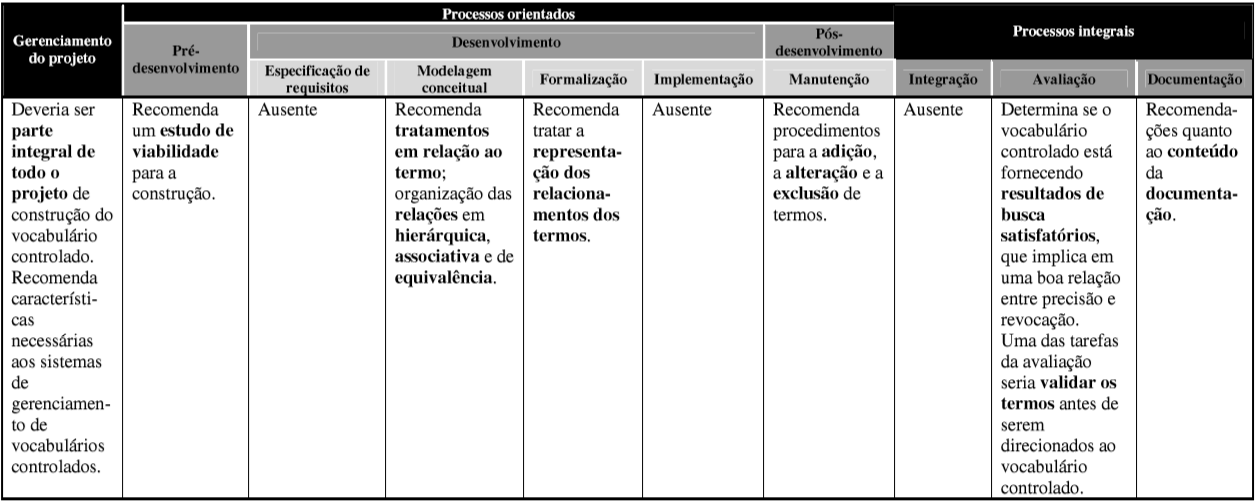
\includegraphics[scale=0.4]{Figuras/13.png} 
% \caption[Tabela abreviada da norma ANSI/NISO Z39.19-2005]
% {Tabela abreviada da norma ANSI/NISO Z39.19-2005. Fonte: \cite{DanielaLucas2008}}
% \end{figure}
% 
% \begin{figure}[h]
% \centering 
% 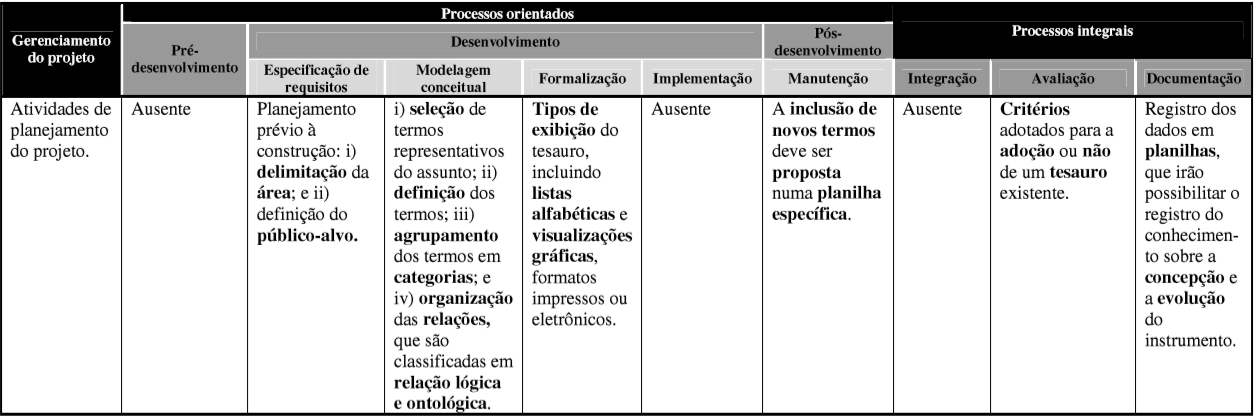
\includegraphics[scale=0.4]{Figuras/14.png} 
% \caption[Tabela abreviada da metodologia proposta no manual da BITI]
% {Tabela abreviada da metodologia proposta no manual da BITI. Fonte: \cite{DanielaLucas2008}}
% \end{figure}